\documentclass[12pt]{article}
\usepackage{pictex,amsmath,amsfonts,fullpage,amssymb,amsthm}
\usepackage{graphics,graphicx}
\usepackage{fancyhdr}
\usepackage{multirow}
\usepackage{algorithm,algorithmic,listings}

\setlength{\voffset}{-0.25in}
\setlength{\headsep}{+0.5in}
\setlength{\parskip}{1em}
\setlength{\parindent}{0em}

\def\vu{\mathbf{u}}
\def\vv{\mathbf{v}}
\def\vs{\mathbf{s}}
\def\vb{\mathbf{b}}
\def\vw{\mathbf{w}}

\renewcommand{\implies}{\rightarrow}
\renewcommand{\lor}{\vee}
\renewcommand{\land}{wedge}
\renewcommand{\iff}{\leffrightarrow}
\newcommand{\TRUE}{\mathbf{T}}
\newcommand{\FALSE}{\mathbf{F}}
\newcommand{\universe}{\mathcal{U}}

\usepackage{xcolor}
\usepackage{mdframed}
\usepackage[utf8]{vietnam}
\usepackage[utf8]{inputenc}
\usepackage[english]{babel}

\newmdenv[linecolor=red,skipabove=\topsep,skipbellow=\topsep,leftmargin=5pt,rightmargin=-5pt,innerleftmargin=5pt,innerrightmargin=5pt]{mybox}

\begin{document}
\begin{center}
\textbf{Some Python code}
\end{center}
\section{Subsetting List}
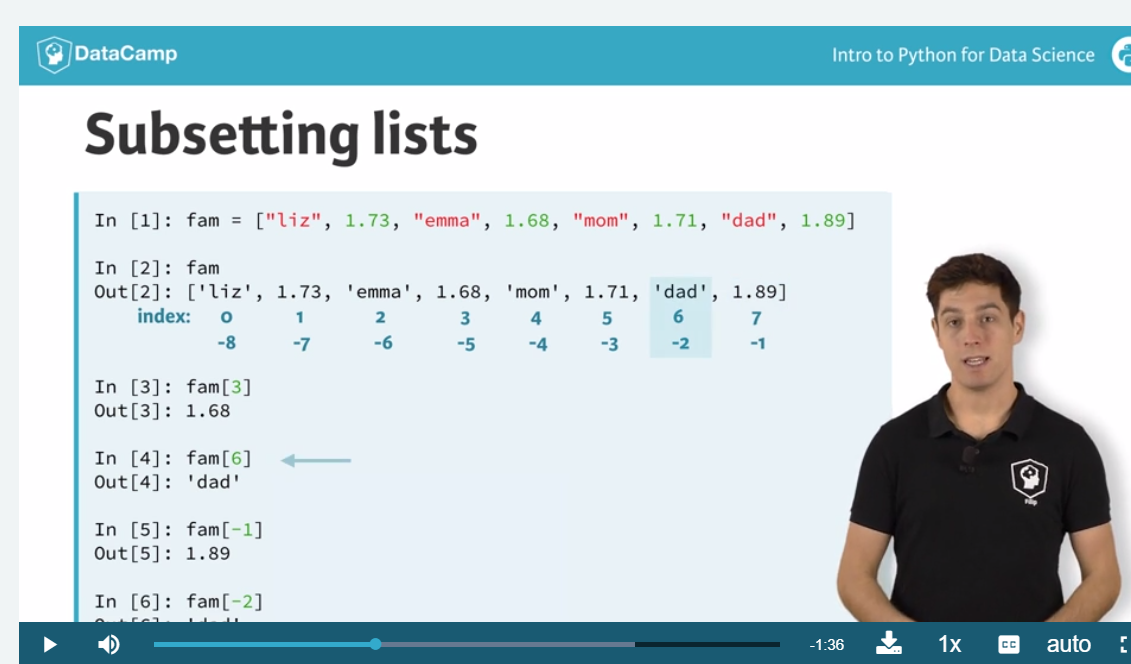
\includegraphics[scale=0.8]{hinh}
\textbf{List Slicing :}
\begin{lstlisting}
list[`liz', 1.73, `emma', 1.68, `mom', 1.71, `dad', 1.89]
list[3:5]
//Terminate:
[1.68, `mom'
\end{lstlisting}
\section{Add to list}
\begin{lstlisting}
# Create the areas list and make some changes
areas = ["hallway", 11.25, "kitchen", 18.0, "chill zone", 20.0,
         "bedroom", 10.75, "bathroom", 10.50]

# Add poolhouse data to areas, new list is areas_1
areas_1 = areas + ["poolhouse", 24.5]
print(areas_1) 

# Add garage data to areas_1, new list is areas_2
areas_2 = areas_1 + ["garage", 15.45]
print(areas_2)
\end{lstlisting}
\section{Delete list element}
\begin{lstlisting}
x = ["a", "b", "c", "d"]
del(x[1])
print(x)
\end{lstlisting}
Then we have:[`b',`c',`d']
\section{Inner workings on lists}
\begin{lstlisting}
# Create list areas
areas = [11.25, 18.0, 20.0, 10.75, 9.50]

# Create areas_copy
areas_copy = areas

# Change areas_copy
areas_copy[0] = 5.0

# Print areas
print(areas)
\end{lstlisting}
\end{document}

